\documentclass[border=10pt]{standalone}

\usepackage{tikz}
\usepackage{tikzsymbols}
\usetikzlibrary{calc,patterns,shapes.geometric}

\def\centerarc[#1](#2)(#3:#4:#5){\draw[#1] ($(#2)+({#5*cos(#3)},{#5*sin(#3)})$) arc (#3:#4:#5);}

\begin{document}
	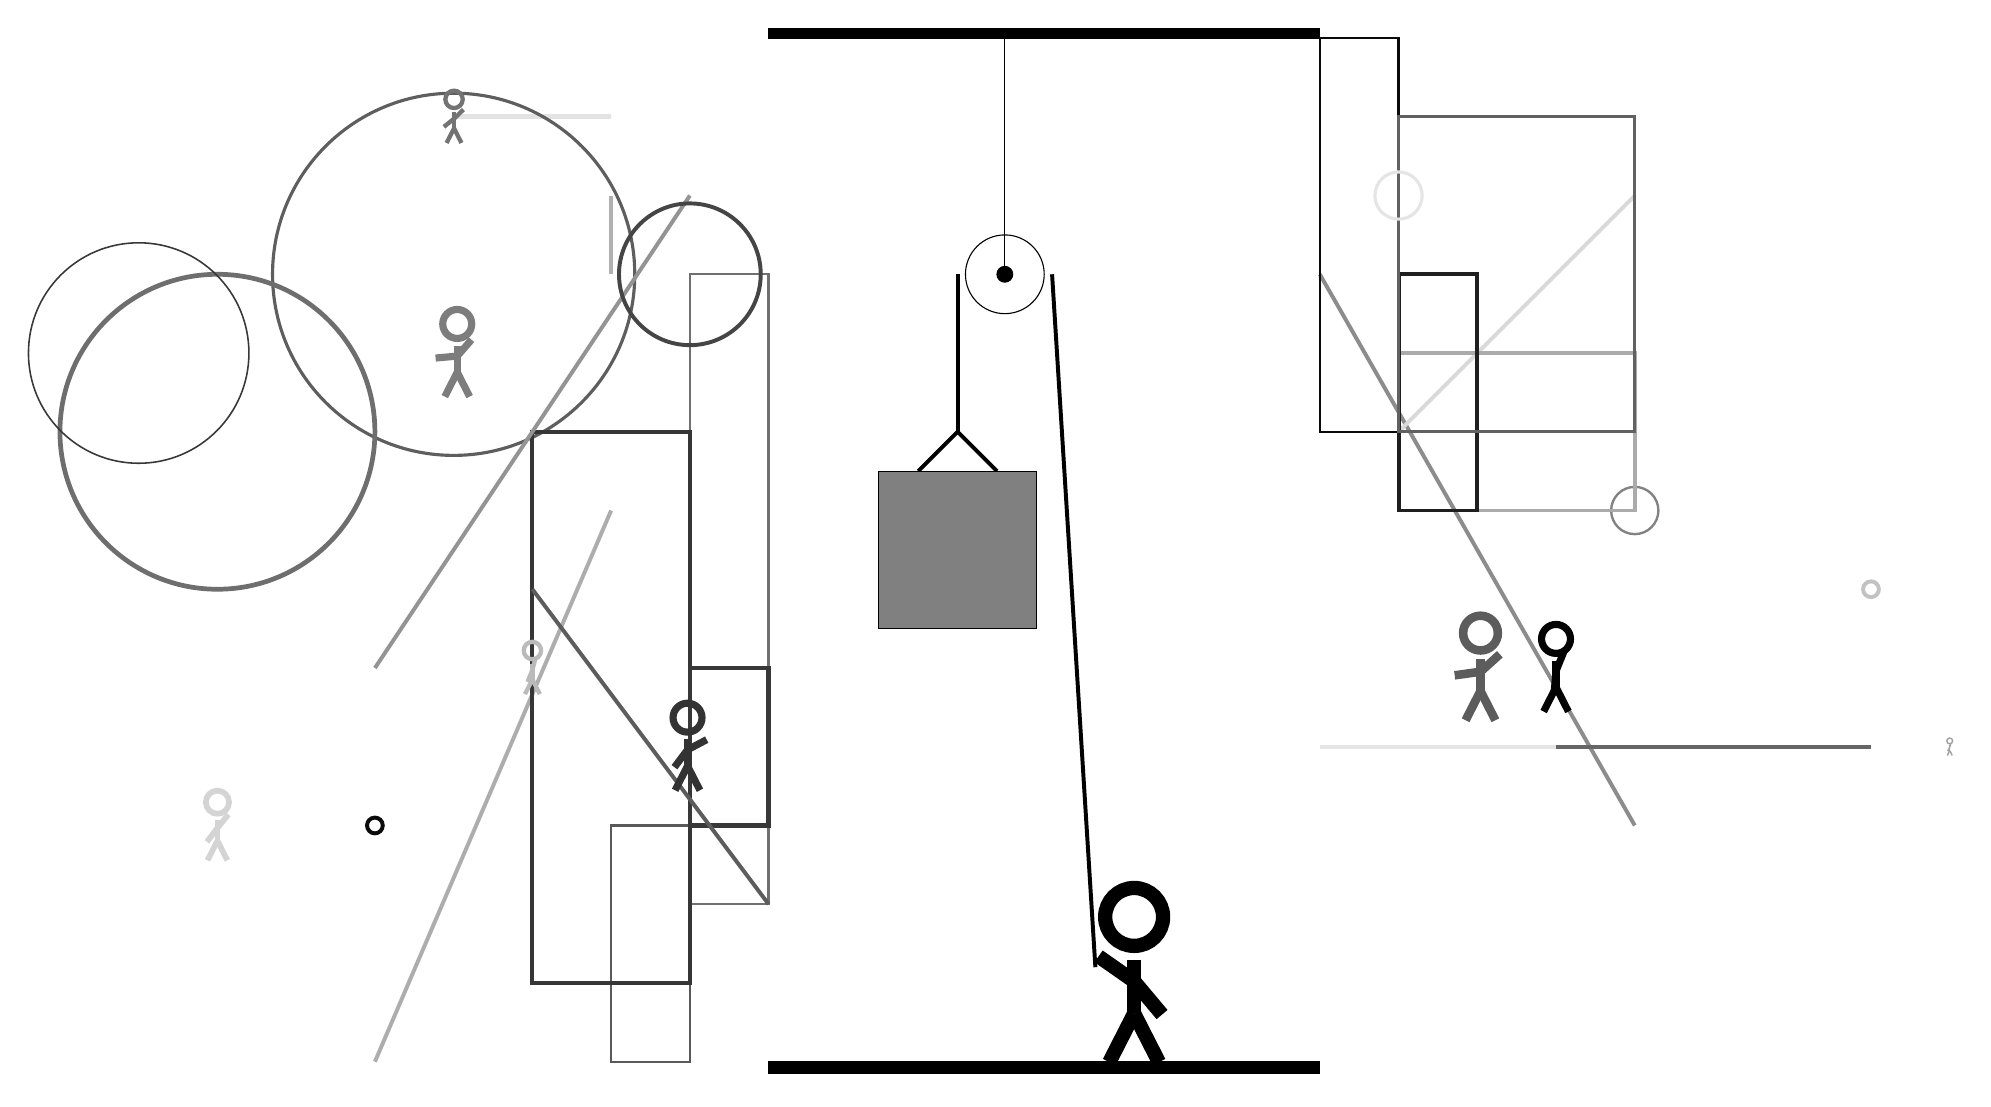
\begin{tikzpicture}
		%%%%% START %%%%%
		
		\draw[fill=black] (-2, 10) rectangle (5, 10.125);
		
		\draw[line width=0.5mm, color=black!45](5, 7) -- (9, 0);
		
		\draw[line width=0.5mm, color=black!60](5, 1) -- (12, 1);
		\draw[line width=0.5mm, color=black!15](9, 8) -- (6, 5);
		\draw[line width=0.6mm, color=black!11] (-4, 9) rectangle (-6, 9);
		\draw[line width=0.3mm, color=black!65] (-4, -3) rectangle (-3, 0);
		
		\draw[line width=0.3mm, color=black!56] (-2, -1) rectangle (-3, 7);
		\node[line width=0.7mm, color=black!51] at (-6, 6) {\Strichmaxerl[5][5][49]};
		
		\node[line width=0.4mm, color=black!37] at (13, 1) {\Strichmaxerl[1][61][74]};
		\draw [line width=0.3mm, color=black!49](9, 4) circle (0.3);
		\draw[line width=0.5mm, color=black!32](-4, 4) -- (-7, -3);
		
		\draw [line width=0.4mm, color=black!63](-6, 7) circle (2.3);
		
		\node[line width=0.3mm, color=black!55] at (-6, 9) {\Strichmaxerl[3][39][44]};
		\draw[line width=0.5mm, color=black!79] (-3, 5) rectangle (-5, -2);
		
		\draw[line width=0.5mm, color=black!33] (6, 4) rectangle (9, 6);
		\draw[line width=0.5mm, color=black!88] (7, 4) rectangle (6, 7);
		\draw [line width=0.6mm, color=black!57](-9, 5) circle (2.0);
		
		\draw[line width=0.3mm, color=black!96] (6, 5) rectangle (5, 10);
		\draw[line width=0.6mm, color=black!78] (-2, 0) rectangle (-3, 2);
		\draw[line width=0.5mm, color=black!42](-3, 8) -- (-7, 2);
		\draw[line width=0.5mm, color=black!64](-2, -1) -- (-5, 3);
		\draw[line width=0.4mm, color=black!62] (6, 9) rectangle (9, 5);
		
		\draw [line width=0.4mm, color=black!10](6, 8) circle (0.3);
		
		\node[line width=0.5mm, color=black!17] at (-9, 0) {\Strichmaxerl[4][53][51]};
		\node[line width=0.2mm, color=black!27] at (-5, 2) {\Strichmaxerl[3][68][75]};
		\node[line width=0.2mm, color=black!64] at (7, 2) {\Strichmaxerl[6][8][42]};
		\draw[line width=0.5mm, color=black!10](5, 1) -- (8, 1);
		\draw [line width=0.5mm, color=black!24](12, 3) circle (0.1);
		\node[line width=0.3mm, color=black!99] at (8, 2) {\Strichmaxerl[5][85][68]};
		\draw [line width=0.2mm, color=black!78](-10, 6) circle (1.4);
		
		\draw [line width=0.5mm, color=black!96](-7, 0) circle (0.1);
		\draw[line width=0.5mm, color=black!31](-4, 7) -- (-4, 8);
		\draw [line width=0.5mm, color=black!73](-3, 7) circle (0.9);
		\node[line width=0.2mm, color=black!80] at (-3, 1) {\Strichmaxerl[5][53][28]};
		
		\draw (1, 7) circle (0.5);
		\draw[fill=black] (1, 7) circle (0.1);
		\draw (1, 10) -- (1, 7);
		
		\draw[line width=0.5mm] (-0.1, 4.5) -- (0.4, 5.0) -- (0.9, 4.5);
		\draw[fill=black!50] (-0.6, 4.5) rectangle (1.4, 2.5);
		
		\draw[line width=0.5mm] (0.4, 7) -- (0.4, 5.0);
		\centerarc[line width=0.5mm](1, 7)(0:180:0.6);
		\draw[line width=0.5mm](1.6, 7) -- (2.15, -1.8);
		
		\node at (2.6, -1.9) {\Strichmaxerl[10][-35][-50]};
		
		\draw[fill=black] (-2, -3) rectangle (5, -3.15);
		
		%%%%% END %%%%%
	\end{tikzpicture}
\end{document}